% !TEX root = ../main.tex
% !TeX spellcheck = fr_FR

\chapter{Expériences automatisées et reproductibles} % (fold)
\label{cha:automated_and_reproducible_experiments}

\epigraph{It doesn't matter how beautiful your theory is, it doesn't matter how smart you are. If it doesn't agree with experiment, it's wrong.}{Richard Feynman}

\minitoc

\textbf{Contribution} Démonstration d'une méthodologie reproductible et
automatisée d'expérience sur réseau de capteurs démontrant la possibilité via
Contiki et Cooja d'avoir une méthode de développement locale utilisant
l'émulation puis de déployer le même code sur Iotlab et d'avoir des cycles
d'itérations courts entre l'implémentation et le test sur système réel.

Il faut annoncer le plan

% subsection contributions (end)

\section{Makesense} % (fold)
\label{sec:makesense}


\subsection{Motivations \& Écosystèmes} % (fold)
\label{sec:automation_motivation}

\textbf{Recherche reproductible} Le développent des testbeds et des outils de
simulations rende la recherche plus facile. Cependant il est encore rare de
trouver un article partageant les sources et les fichiers nécessaires aux
résultats qu'il annonce. Ce paradoxe a été repéré dans des domaines très
variés \cite{peng2011reproducible, wilson2014best}. Comment s'assurer que les
résultats annoncés dans un article sont vérifiables et peuvent être partagés.

Nous présenterons dans ce chapitre la méthodologie que nous avons utilisé pour
obtenir les résultats précédents et nous introduirons
Makesense~\cite{leone2013makesense}.

\begin{figure}
%\begin{bigcenter}
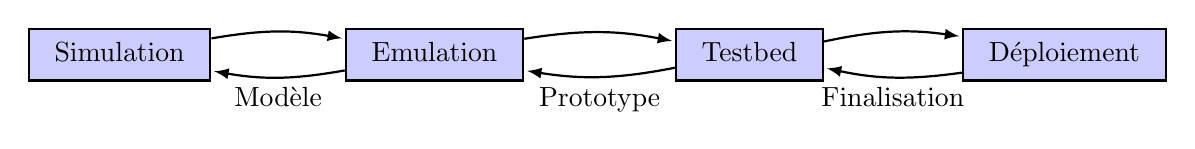
\begin{tikzpicture}[->,>=latex,shorten >=1pt,auto,node distance=3cm,
  thick,main node/.style={fill=blue!20,draw}]

  \node[main node] (sim) at (0,0) {\begin{tabular}{c}Simulation\end{tabular}};
  \node[main node] (emu) at (4,0) {\begin{tabular}{c}Emulation\end{tabular}};
  \node[main node] (testbed) at (8,0) {\begin{tabular}{c}Testbed\end{tabular}};
  \node[main node] (final) at (12,0) {\begin{tabular}{c}Déploiement\end{tabular}};

  \path
    (sim) edge[bend left=10] (emu)
    (emu) edge [bend left=10] node[below] {Modèle} (sim)

    (emu) edge[bend left=10] (testbed)
    (testbed) edge [bend left=10] node[below] {Prototype} (emu)

    (testbed) edge[bend left=10] (final)
    (final) edge [bend left=10] node[below] {Finalisation} (testbed)

;
\end{tikzpicture}
%\end{bigcenter}
\caption{Cycles de développement}\label{fig:automation:development_workflow}
\end{figure}

Le développement d'une expérience passe par plusieurs étapes
\ref{fig:automation:development_workflow}. Selon l'étape, les contraintes et
les attentes sont différentes. Comme montré dans la
figure~\ref{fig:automation:comparatif}, en phase de simulation, il est attendu
d'avoir des preuves de concepts rapides et facilement modifiables. Le réalisme
est souvent modeste du à des hypothèses simplificatrices qui rendent le
dévelopment aisé. Le contrôle sur l'expérience est total, les résultats sont
faciles à partager et la reproductibilité est garantie si les paramètres
aléatoires comme les graines génératrices sont fixées. À l'inverse dans le cas
d'un testbed, le réalisme est fort, les problèmes d'intégration sont nombreux,
variés et difficilement prévisibles. Certaines plateformes offrent des traces
détaillées de l'expérience mais aucune ne peuvent garantir que deux
expériences seront reproduites à l'identique.

\begin{figure}[tb]
  \centering
  \begin{tabular}{|c|c|c|c|c|}
    \hline  & Realisme & Contrôle & Déploiement & Reproductibilité \\ 
    \hline Testbed (Iotlab) & Elevé & Faible & Faible & Faible \\ 
    \hline Emulation (Cooja - motes) & Moyen & Moyen & Moyen & Moyen \\ 
    \hline Simulation (Cooja - Radio) & Faible & Elevé & Elevé & Elevé \\ 
    \hline 
  \end{tabular} 
  \caption{Evaluation des solutions expérimentales}
  \label{fig:automation:comparatif}
\end{figure}

Comme nous pouvons le voir dans le Table~\ref{fig:automation:comparatif}, il
existe différentes solutions pour développer et évaluer une expérience. Cooja
\cite{cooja} et Contiki~\cite{dunkels2004contiki}

\subsection{Etat de l'art} % (fold)
\label{sub:etat_de_l_art}

Evaluating applications and protocols through simulation always follow the
same workflow from the simulation parameters definition to the creation of
graphs that represent performance under different conditions. Yet, no generic
tool really provides a way to automate the whole process and people often rely
on ad-hoc scripts. Some tools such as NEPI \cite{lacage2010nepi} focus on the
interaction between testbeds, but do not address wireless sensor network
platforms and hence, their architecture may be too complex for constrained
devices.

\textbf{Tools rather than complete solution} Plutôt que de créer un framework
ayant pour tâche étroite de gérer nos simulations. Utiliser un ecosystème de
logiciels ayant des communautés larges et ancrées dans les problématiques
scientifique est un choix. langage facile a comprendre et pas une \ac{DSL}
construite pour résoudre un seul problème. Misé sur une communauté vivante
plutôt que sur un papier prophétique. Nepi \cite{lacage2010nepi} est basé sur
l'idée d'une abstraction du testbed au profit d'objets génériques. Le problème
de cette approche est qu'elle repose essentiellement sur des adaptateurs.
Cooja \cite{cooja} et  Iotlab \cite{fleury2015fit} était absent de la liste
des adaptateurs proposés. En outre, l'API de IoTlab étant très simple et
maintenue nous l'avons utilisé directement.


% subsection etat_de_l_art (end)

\subsection{Architecture} % (fold)
\label{sub:architecture}

Makesense rassemble les paramètres, fonctions et résultats dans un seul et
même Jupyter notebook. Ce fichier est un fichier texte au format \ac{JSON}. Ce
fichier contient par exemple les graines des générateurs de nombre aléatoires, 
les portées de transmission et de reception.

Comme ce fichier texte rassemble l'ensemble des paramètre il est facile de le
modifier et de l'utiliser comme modèle pour gérerer d'autres expériences au
sein d'une même campagne de simulations. La modification de ce fichier via un
éditeur de texte serait très fastidieuse. Jupyter est équipé d'un serveur
permettant de générer un rendu HTML du notebook. Ainsi, n'importe quel
naviagateur web permet de visualiser et modifier l'ensemble du fichier
décrivant l'expérience. Le notebook contient toute l'intelligence et la
présentation.

Un notebook est constitué de cellules qui peuvent contenir du texte, de
l'audio, de la vidéo ou bien des snippets de code. Jupyter~\cite{PER-GRA:2007}
découple le moteur d'execution du format du JSON. Ainsi il est possible
d'utiliser un moteur différent tel que Julia ou bien R.

Lorsqu'une cellule de texte est rendue, le \LaTeX{} et le markdown contenu  dans
cette cellule est rendue à l'utilisateur. Ainsi il est possible d'introduire
des formules de \LaTeX{} et avoir un rendu de formules mathématiques complexes
fonctionnant sur n'importe quel navigateur moderne.

\textbf{Simplicité} Utiliser un seul et même langage pour organiser nos
expérience et traitements est un atout. Plutôt que de chercher à coller des
composants différents utilisant différents language et des outils lourds tel
que matlab et consorts, nous avons privilégié les solutions ouvertes, légères
et agnostiques. Python dispose de cette versatilité et dispose de communautés
ancrées dans la recherche scientifique et offre de nombreuses bibliothèques.

\section{Construction d'une expérience reproductible} % (fold)
\label{sub:steps}

\begin{figure}[tb]
  \centering
  \includegraphics[]{img/makesense_scheme.pdf}
  \caption{Schéma général de l'enchainement des étapes dans Makesense}
  \label{fig:makesense:schema}
\end{figure}

\begin{figure}
%\begin{bigcenter}
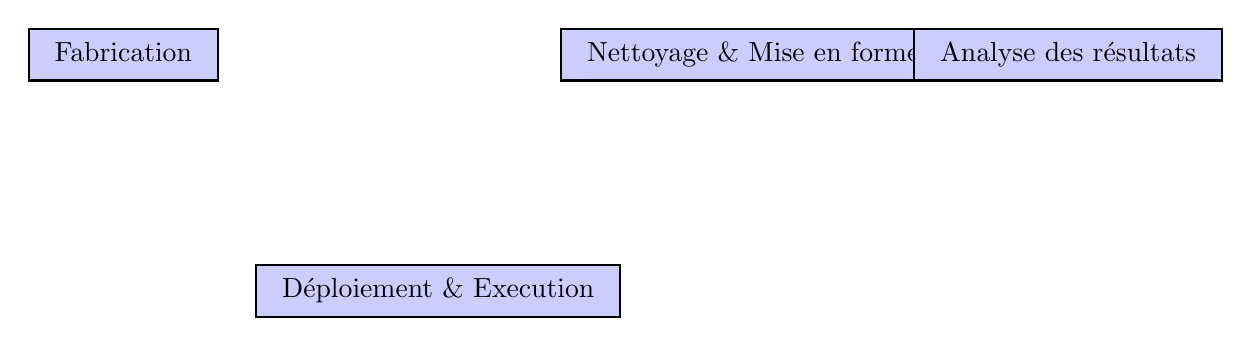
\begin{tikzpicture}[->,>=latex,shorten >=1pt,auto,node distance=3cm,
  thick,main node/.style={fill=blue!20,draw}]

  \node[main node] (make) at (0,0) {\begin{tabular}{c}Fabrication\end{tabular}};
  \node[main node] (deploy-exec) at (4,-3) {\begin{tabular}{c}Déploiement \& Execution\end{tabular}};
  \node[main node] (parse) at (8,0) {\begin{tabular}{c}Nettoyage \& Mise en forme\end{tabular}};
  \node[main node] (analyze) at (12,0) {\begin{tabular}{c}Analyse des résultats\end{tabular}};

  % \path
  %   (sim) edge[bend left=10] (emu)
  %   (emu) edge [bend left=10] node[below] {Modèle} (sim)

  %   (emu) edge[bend left=10] (testbed)
  %   (testbed) edge [bend left=10] node[below] {Prototype} (emu)

  %   (testbed) edge[bend left=10] (final)
  %   (final) edge [bend left=10] node[below] {Finalisation} (testbed)

;
\end{tikzpicture}
%\end{bigcenter}
\caption{Cycles de développement}\label{fig:automation:development_workflow}
\end{figure}


Afin d'illustrer l'intérêt de makesense et plus généralement de l'ecosystème
Python, nous allons exposer comment organiser une expérience utilisant Contiki
\cite{dunkels2004contiki} et le simulateur cooja \cite{cooja}.

\subsection{Préparations préalables - Compilation des systèmes contraints} % (fold)
\label{sub:subsection_name}

\textbf{Description de l'étape} Il s'agit de  l'étape ``make'' dans la
figure~\ref{fig:makesense:schema}. Il faut parler ici du fait que les plateformes
utilisées sont nombreuses et qu'il faut parfois avoir plusieurs firmwares compilés.

Il faut en outre parler du fait que l'on veut parfois créer des environnements
de simulations dynamiquement (par exemple généré un graphe aléatoire avec un
nombre arbitraire de noeuds). 

\textbf{Méthodes \& outils utilisés} Jinja2 \cite{jinja2} est un moteur de
template qui permet de générer des fichiers textes à partir de modèles de
référence. Ce moteur est particulièrement utile pour générer une série de
fichiers sources pour nos noeuds disposant de différentes variables/programmes
différents selon les circonstances.

\textbf{Justification de cette méthode} Un cas d'usage classique de cette
étape est de créer une ``campagne'' de simulations avec des noeuds ayant
differentes fonctionnalités. Dans le cas où les noeuds sont très contraints il
peut être vraiment difficile de générer le système d'exploitation

L'étape de compilation peut et doit être automatisée. En effet, il n'est pas
rare que les noeuds réels disponibles soient sur des plateformes différentes
et doivent être adaptés.

\subsection{Déploiement \& Execution - rappatriement}

\textbf{Description de l'étape} Il s'agit de  l'étape ``deploy'' et
``run\_exp'' dans la figure~\ref{fig:makesense:schema}.

Les destinations des noeuds peuvent changer. Dans le cas de Iotlab il y a plusieurs
noms différents selon le site du testbed utilisé.

Il est nécessaire de gérer plusieurs outils parallèlement (génération de
traffic, lancement des loggeurs, lancement du simulateur, vérification et
monitoring des connexions).
Il faut gérer le fait que dans le cas d'un testbed il est nécessaire de
faire des reservations et que le lancement d'une commande ne veut pas nécessairement
dire que l'expérience va être effectué immédiatement.

Problématiques assez complexes de réaction à des évenements asynchrones.

\textbf{Méthodes \& outils utilisés} Fabric \cite{fabric} est une bibliothèque
permettant de transmettre et d'executer des programmes sur des plateformes
distantes. Dans le cas de la plateforme IoTlab \cite{fleury2015fit}, l'envoi
et le rappatriements des différentes traces a été automatisé afin de pouvoir
reproduire n'importe quelle experience lancée.

\inputminted{python}{snippets/fabric.py}

\textbf{Justification de cette méthode} Il serait possible de lancer des
commandes de manière séquentielle et obtenir le même résultat. Cependant
intégrer directement au sein de nos scripts des moyens de regénérer à la volée
des fichiers de configurations différents selon les testbeds utilisés est une
grande aide. De plus la possibilités de récupérer de manière parallelisée les
résultats obtenus sur différents testbeds accélère considérablement les tâches
répétitives.

L'abstraction est également une propriété importante. Dans notre cas, il est
intéressant de pouvoir avoir une abstraction sur où va se passer l'expérience
et faire en sorte que le rangement des résultats soit indépendant du lieu où
l'expérience s'est produite. L'execution peut avoir lieu dans plusieurs
endroits. Que ça soit dans un simulateur ou sur des noeuds réels. L'execution
d'une simulation peut nécessiter une série d'intéraction. Par exemple une
génération de traffic, des processus de supervision des processus et des
communications ou encore la relance de services qui ont des pannes.

\subsection{Mise en forme des résultats intermédiaires}

\textbf{Description de l'étape}  Il s'agit de  l'étape ``parse''  dans la
figure~\ref{fig:makesense:schema}  \textbf{Il faut faire cette étape dans un
nouveau schéma de makesense.}

Parler des conversions d'unités, de normalisation de valeurs, de mise en place
de tags sur les différents paquets pour bien comprendre quels paquets sont en
jeu à chaque instant, de la mise en forme de certains résultats tel que le
PCAP. La transformation des adresses mac vers des identifiants plus facilement
compréhensibles

Dans le cas de système très contraint, il est possible que des logs explicites
soit remplacés par des écritures compressés qui rendent la lecture des
résultats plus difficile. Cette étape permet de retransformer toutes les meta
données.

Effecturer des assainissement en fonction du type de paquet (par exemple
classifier des paquets selon les champs qu'ils comportent).

Formaliser certains messages vers des structures de données qui rendent
l'analyse postérieur facile. Par exemple certains messages de parents peuvent
être lus et transformer vers des structures de données de type graphe
connecté.

\textbf{Méthodes \& outils utilisés} tshark \cite{tshark} est un outil en
ligne de commande permettant d'extraire une série de statistiques en
provenance d'un fichier \ac{PCAP}. La concurrence vis a vis de ce secteur
d'analyse est essentiellement Wireshark. Cependant Wireshark requiert une
interface graphique en plus d'être relativement lent pour le recalcul de
filtres et l'extraction intelligente d'attributs. L'avantage de tshark et de
transformer une trace en un format texte qui offre une plus grande facilité et
une plus grande versatilité.

\inputminted{python}{snippets/parsing.py}

\textbf{Justification de cette méthode} Il serait possible d'utiliser des
outils graphiques comme Wireshark pour pouvoir faire de l'exploration ad-hoc.
Bien que cette méthode soit utile durant les phases d'exploration et de
consolidation du protocole expérimental, le maintenir durant les phases de
production ralenti la production de résultats. Les interfaces graphiques ne
sont pas conçues pour des traitements massifs d'information. En outre, les
changements de filtres dans Wireshark nécessite des recalculs sur l'ensemble
des fichiers capturés. À l'inverse une fois que les données essentielles sont
mises dans un fichier texte. On se retrouve sur des données qu'il est facile
de filtrer avec les outils classiques.

\subsection{Analyse des résultats}

\textbf{Description de l'étape}  Il s'agit de  l'étape ``analyze''  dans la
figure~\ref{fig:makesense:schema}
\textbf{Il faut mettre le nom des étapes en français!!!}

Calculs divers sur le graphe (Profondeur,
connexité) Statistiques diverses sur le nombre de paquets, le type de traffic,
les pertes de paquets. C'est plus généralement dans cette étape que va se
faire la recherche et la production de résultats qualitatifs et quantitatifs
sur notre étude.

\textbf{Méthodes \& outils utilisés} Pandas \cite{mckinney-proc-scipy-2010}
est une bibliothèque écrite pour le langage de programmation Python permettant
la  manipulation et l'analyse des données. Elle propose en particulier des
structures de données et des opérations de  manipulation de tableaux
numériques et de séries temporelles. Pandas est un logiciel libre sous licence
BSD.

\inputminted{python}{snippets/pandas.py}

\textbf{Justification de cette méthode} Il serait possible d'utiliser des
outils de filtres texte tel que awk ou sed. Ils sont utiles dans des cas très
simples mais dès qu'il s'agit de grouper et de faire des aggrégations leur
utilisation peut devenir difficile. En outre, la syntaxe de ces outils est
moins claire que celle de pandas qui s'inspire de \ac{SQL} afin d'avoir un
formalisme lisible.

Dans notre cas d'exploration du réseau, nous avons également utilisé NetworkX.
Cette bibliothèque nous permet de gérer les données liées à des graphes. Dans
nos cas, nous voulions avoir une représentation du \ac{DODAG} \ac{RPL}, être
capable de calculer les plus courts chemins entre un nœud et la racine du
\ac{DODAG}. Networkx nous apporte des facilités de calcul et de représentation
graphique nous permettant de visualiser l'ensemble des liens pertinents dans
le réseau.

\subsection{Présentation des résultats}

\textbf{Description de l'étape} Moment de partage dans l'équipe. On peut
exposer les idées

Production de graphes qui vont être après inséré dans une publication

Consultation et Modification de paramètres facile sans connaitre tous les
détails de l'implémentation

\textbf{Méthodes \& outils utilisés} matplotlib \cite{Hunter:2007} est une
bibliothèque de graphisme permettant de programmer un graphe.
jupyter  / HTML export / Ajout de markdown et de formules \LaTeX{}.

\textbf{Justification de cette méthode}  L'intérêt d'utiliser ce genre de
bibliothèque plutôt que des solutions spécialisées tel que Gnuplot
\cite{Gnuplot_4.4} vient du simple fait qu'elle peut être intégré directement
à la suite de pandas. En effet, il est possible de chaîner des opérations et
obtenir un graphe rapidement a la suite d'une série de filtres et
d'aggrégations.

\inputminted{python}{snippets/matplotlib.py}

Nous obtenons ainsi en une ligne de code, un graphe représentant l'histogramme
du nombre de paquets.

\textbf{Justification de cette méthode} Au lieu de créer un rapport qui soit un
ensemble de fichiers graphes ou bien d'une page web basique, on peut créer un
rapport qui permette de ré-exécuter certaines portions de code. L'annotation et
la modification des textes qui est en marge des résultats permet d'avoir une
façon beaucoup plus lisible de partager des résultats.

\subsection{Garanties de reproductibilité par intégration continue} % (fold)
\label{sub:performance_evaluation}

\textbf{Description de l'étape} L'intégration continue est un ensemble de
pratiques utilisées en production de logiciel qui consiste à vérifier que
chaque modification apportée au code source ne modifie pas la correction du
code et n'introduit pas de régression. Le principal but de cette pratique est
de détecter les problèmes et les erreurs afin de les corriger au plus tôt.

Dans le cas d'expériences se déroulant sur un testbed, il serait très complexe
de s'assurer de la reproduction. En effet, l’environnement du testbed est un
système réel changeant. De plus, le matériel du testbed peut être
indisponible, remplacé, altéré.

Dans le cas de simulations, le but est d'assurer que l’environnement de
simulation est reproductible. Ainsi, il est possible pour n'importe quel
lecteur de reproduire les conditions dans lesquels les expériences ont étées
executées et produites. Dans le cas d'expériences aléatoires comme les notres,
un simulateur peut être complètement reproductible dès lors que ses graines de
générateurs de nombres aléatoires ont été fixés. À ce moment-là a jeu de
paramètres égaux les résultats sont constants.

\textbf{Méthodes \& Outils utilisés} Travis-ci \cite{travis} est un service
d'intégration continue qui permet de construire et d’exécuter une série de
tests lorsqu'une modification proposée ou effective du code a lieu. Lorsque la
série de tests est terminée on peut ainsi vérifier qu'aucune régression des
fonctionnalités n'a été commise. Ce service utilisé entre autre pour tester le
système Contiki \cite{contiki_travis} peut l'être pour reproduire des
expériences. Ainsi nous avons pu construire une démonstration présentant les
différentes étapes présentées dans ce chapitre et les avons exécuté sur cette
plate-forme \cite{leone2014demo}. Le fait que Travis soit une structure
indépendante et ouverte renforce le fait que n'importe qui pourrait refaire
l'expérience et s'assurer de nos résultats.

\textbf{Justification de cette méthode} La possibilité de vérifier rapidement
qu'une expérience a bel et bien fonctionné via un tiers de confiance est un
bon signe et un gage sur le travail effectué. Une fois que cette vérification
a été faite il est aisé de trouver l'environnement logiciel qui a permis la
production des résultats pour être capable de partir de cette environement
afin de le modifier à nouveau et d'itérer rapidement afin de produire de
nouveaux résultats.

\section{Conclusion \& Perspectives} % (fold)
\label{sec:conclusion}

\begin{itemize}

  \item La reproductibilité d'une expérience est une question complexe mais
    doit devenir une problématique de premier plan

  \item A l'inverse d'autres disciplines scientifiques, l'informatique et le
    réseau jouissent d'une situation enviable où le cout pour reproduire une
    expérience est souvent modeste

  \item de nombreux outils existent en licence libre ou bien des plateformes
    intégrés tel que jenkins ou travis.

  \item Reconnaissance par la communauté: Des plateformes de partage de travaux
    scientifiques tel que hal permettent d'héberger les fichiers nécessaires.

\end{itemize}

\textbf{Perspectives}

\begin{itemize}

  \item Prise de conscience et lobbying
  
  \item Développement d'outils et de plateformes qui vont dans ce sens (parler
    de iotlab)

\end{itemize}

% section conclusion (end)

% chapter automated_and_reproducible_experiments (end)
